% klasa report,jednostronny
\documentclass[a4paper, 11pt, oneside]{article}

% kodowanie
\usepackage[utf8]{inputenx}
\usepackage[T1]{fontenc}
\usepackage{listings}


% czcionka Arial
\usepackage{helvet}
\renewcommand{\familydefault}{\sfdefault}

% jezyk tekstu
%\usepackage{polski}
%\usepackage[polish]{babel}

% marginesy
\usepackage[inner=30mm,outer=20mm,top=25mm,bottom=25mm]{geometry}

% interlinia
\linespread{1.15}

% paczka do zarzadza headerami i footerami; ustawienie numeracji w dolnym zewnetrznym rogu
\usepackage{fancyhdr}   
\pagestyle{fancy}
\fancyhead{}% clear headers
\fancyfoot{}% clear footers
\renewcommand{\headrulewidth}{0pt}% eliminate horizontal line
\fancyfoot[RO, LE]{\thepage}
% redefinicja stylu plain (zeby na stronach z tytulem rozdzialu tez bylo dobrze
\fancypagestyle{plain}{%
  \fancyhf{}%
  \fancyfoot[RO, LE]{\thepage}%
  \renewcommand{\headrulewidth}{0pt}% Line at the header invisible
  \renewcommand{\footrulewidth}{0pt}% Line at the footer visible
}

% Akapit do wyboru:

% wcięcie 5mm
% \usepackage{indentfirst}
% \setlength{\parindent}{5mm}
% \setlength{\parskip}{0ex} 

% odstep 4 pomiedzy akapitami
 \setlength{\parindent}{0mm}
 \setlength{\parskip}{2ex} 


% paczka do rysunkow
\usepackage{graphicx}
\usepackage{float}
% foldery z rysunkami
\graphicspath{ {Rysunki/} {Wykresy/} }
% domyslnie numeracja wg rozdzialow
% ponizej ciagla w pracy
% \usepackage{chngcntr}
% \counterwithout{figure}{chapter}

%ponizej zeby podpisy mialy dobry rozmiar i byly gdzie trzeba w rysunkach
\usepackage{caption}
\DeclareCaptionFormat{myformat}{\fontsize{9}{10}\selectfont#1#2#3}
\captionsetup{format=myformat}
\captionsetup[figure]{slc=off}

% paczki do robienia ladnych tabel, ustawienie podpisow itd, zmiana tablica na tabela
\usepackage{booktabs}
\usepackage[svgnames,table]{xcolor}
\usepackage{threeparttable}
\captionsetup[table]{justification=justified,singlelinecheck=false}
\usepackage{pifont}

%\renewcommand{\tablename}{Tabela}

% zmiana czcionek w (pod)rozdziałach
\usepackage{anyfontsize}
\usepackage{titlesec}
\titleformat{\chapter}[display]
  {\normalfont\sffamily\fontsize{14}{15}\selectfont\bfseries\color{black}}
  {\chaptertitlename\ \thechapter}{14pt}{\fontsize{14}{15}\selectfont}
\titleformat{\section}
  {\normalfont\sffamily\fontsize{13}{14}\selectfont\bfseries\color{black}}
  {\thesection}{13pt}{}
\titleformat{\subsection}
  {\normalfont\sffamily\fontsize{12}{13}\selectfont\bfseries\color{black}}
  {\thesubsection}{12pt}{}
\titlespacing\chapter{0pt}{0pt plus 4pt minus 2pt}{12pt plus 2pt minus 2pt}
\titlespacing\section{0pt}{6pt plus 4pt minus 2pt}{0pt plus 2pt minus 2pt}
\titlespacing\subsection{0pt}{0pt plus 4pt minus 2pt}{0pt plus 2pt minus 2pt}

% zalaczanie stron pdf
\usepackage{pdfpages}

% generowanie tekstu- do wyrzucenia
\usepackage{lipsum}
%biblioteka matematyczna
\usepackage{ amsmath}
%tikz
\usepackage{pgfplots} 

%Bibliotek do pisania pseudo kodu i kodu
\usepackage{amsmath}
\usepackage{algorithm}
\usepackage[noend]{algpseudocode}

% and optionally (as of Pgfplots 1.3): 
\pgfplotsset{compat=newest} 
\pgfplotsset{plot coordinates/math parser=false} 
\newlength\figureheight 
\newlength\figurewidth

\setcounter{MaxMatrixCols}{20} 


%bibliografia
\usepackage[backend=biber]{biblatex}
\addbibresource{bibs.bib}

%strona tytułowa
\title{%
  SST MISK \\Projekt semestralny \\
  \vspace{5mm}
  \large Monitorowanie celu za pomocą autonomicznej chmury dronów\\
  opracowanie algorytmu kooperacji i symulacja}
\author{Jerzy Baranowski\\Artur Czopor\\Ignacy Ruksza \\Krzysztof Zarzycki }

\date{\today}

\begin{document}

\maketitle
\newpage
\section{Opis projektu}
Celem projektu jest stworzenie i symulacja działania algorytmu sterowania rojem dronów tak by w sposób optymalny formowały ustaloną formację nad wyznaczonym celem. 
\section{Użyte oprogramowanie}

Symulacja wyżej opisanego zadania została wykonana w programie symulacyjnym V-Rep połączonym dedykowanym API ze środowiskiem Matlab. W celu realizacji zadania został zaimplementowany w języku M skrypt optymalizujący trasę przelotu drona w zależności od pozycji celu i roju.  Obiekty latający odwzorowane są w środowisku V-Rep poprzez model symulacyjny “Quadricopter”, który posiada możliwość sterowania poprzez wyznaczenia pozycji docelowej. Model ten został dostarczony przez producenta oprogramowania i ingerencja w jego mechanikę nie jest celem projektu. W celu obejścia ograniczeń modelu trajektoria wyliczana jest wyznaczana poprzez generację punktów docelowych dla kolejnych chwil dla każdego z dronów.

\begin{figure}[H]
\centering
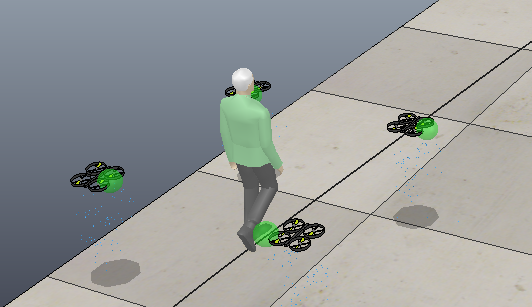
\includegraphics[scale=0.5]{simulation1.png}
\caption{Przykładowa scena z symulatora V-Rep.}

\end{figure}

\section{Opis algorytmu}
Zadaniem, które mają wykonać drony, jest podążanie za poruszającym się człowiekiem w odpowiedniej formacji (kwadrat, wielokąt). Założone zostało, że drony startują z losowych miejsc na planszy i znają położenie zbiega. Muszą one podążyć w jego kierunku optymalną ścieżką, otoczyć go w formacji (która na bieżąco tworzona jest w czasie ich lotu) a następnie go śledzić. Przy tym nie powinno dojść do sytuacji, w której dwa drony zderzą się ze sobą lub ze śledzonym człowiekiem. Zadanie to zostało opisane za pomocą nieliniowego problemu optymalizacji.
\subsection{Problem optymalizacji}
W celu wyznaczenia optymalnej pozycji dronów rozwiązywany jest nieliniowy problem optymalizacji wielu zmiennych z liniowymi i nieliniowymi oraz z równościowymi i nierównościowymi ograniczeniami. Formalny zapis problemu:
\begin{equation}
\operatorname*{min}_x  f(x)=
	\begin{cases}
	\ c(x) \leq 0
	\\
	ceq(x)=0
	\\
	A \cdot x\leq b
	\\
	Aeq \cdot x =beq
	\\
	lb \leq x \leq ub
	\end{cases}
\end{equation}

Uwzględnione zostały tylko więzy opisane funkcją $c(x)$.
Dane problemu:
\begin{itemize}
\item $X$ - zmienna celu
\item $D$ - zadana odległość od celu
\item $d$ - zadana macierz odległości do sąsiada
\item $A$  - minimalna odległość do celu
\item $a$ -  minimalna odległość do sąsiada
\item $L$ - liczba dronów
\end{itemize}
\subsection{Funkcja celu}
Funkcja celu składa się zasadniczo z dwóch członów. Pierwszy z nich odpowiada za ich odległość od śledzonego człowieka. Znana jest pozycja każdego z L dronów, a także położenie celu, w kierunku którego mają lecieć. Zastosowana została więc minimalizacja kwadratu różnicy zadanej odległości między celem, a każdym z dronów.
Drugi człon równania odpowiada za minimalizację odległości pomiędzy dronami. Parametr d to macierz, która określa położenie każdego z dronów w stosunku do jego sąsiada o strukturze:
$$
d=
\begin{bmatrix}
d_{11} &
d_{12} &
\cdots &
d_{1L}\\
d_{21} &
d_{22} &
\cdots &
d_{dL}\\
\vdots &
\vdots &
\ddots & \vdots
\\
d_{L1} &
d_{L2} &
\cdots &
d_{LL}
\end{bmatrix}
$$
gdzie dij – jest odległością między i-tym, a j-tym dronem. W szczególności gdy i=j, to dij wynosi 0.
\newline
\newline
Przykładowo, dla czterech dronów i zadanej formacji o kształcie kwadratu o boku a:
\begin{figure}[H]
\centering
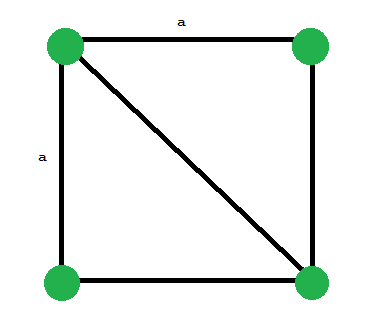
\includegraphics[scale=0.5]{blok_axa.png}
\caption{Formacja dla czterech dronów.}
\end{figure}

Macierz ma postać:
$$
d=
\begin{bmatrix}
0 &
a &
a\sqrt{2} &
a\\
a &
0 &
a &
a\sqrt{2}\\
a\sqrt{2} &
a &
0 & 
a &\\
a &
a\sqrt{2} &
a &
0
\end{bmatrix}
$$
\begin{equation}
f_{target}(x)= \underbrace{\sum_{i=0}^{L}\lbrace D_i^2 - [(X_x -x_{xi})^2+(X_y -x_{yi})^2] \rbrace ^2}_\text{Odległość od celu} +
\underbrace{\sum_{i=0}^{L}\sum_{j=0}^{L}w_i\lbrace d_{ij}^2 -(X_y -x_{yi})^2]\rbrace ^2}_\text{Odległości pomiędzy dronami}
\end{equation}

Opis zmiennych:
\begin{itemize}
\item $X$ - zmienna celu
\item $x$ - zmienne pozycji 
\item $D$ - zadana odległość od celu
\item $d$ - zadana macierz odległości do sąsiada
\item $L$ - liczba dronów
\item $w_i$ - wagi
\end{itemize}

Powyższa funkcja jest wczytywana do procedury optymalizacyjnej rozwiązującej zadanie optymalizacji kwadratowej.
\subsection{Funkcja więzów} 
Funkcja $c(x)$ definiuje więzy narzucone na układ.
\[ f_{constraints}(x)_k=c(x)=\begin{cases} 
      A^2-[(X_x+x_x)^2+(X_y+x_y)^2] & k\in{ 0,..,L-1} \\
      a^2-[(x_{xj}+x_{xi})^2+(x_{yj}+x_{yi})^2] & k\in{ L,..,\binom{L}{2}} 
      
   \end{cases}
\]
Pierwsza część równania opisuję warunek na zachowanie minimalnej  odległości od celu. Druga natomiast opisuję minimalne dopuszczalne odległości pomiędzy parami dronów. Dla $L$ statków powietrznych definiujemy $\binom{L}{2}$ warunków.
Opis zmiennych:
\begin{itemize}
\item $X$ - zmienna celu
\item $x$ - zmienne pozycji
\item $A$  - minimalna odległość do celu
\item $a$ -  minimalna odległość do sąsiada
\item $x_0$ - pozycja początkowa
\item $dx$ - maksymalne przesunięcie
\item $L$ - liczba dronów
\end{itemize}
Powyższa funkcja jest wczytywana do procedury optymalizacyjnej rozwiązującej zadanie optymalizacji kwadratowej.
\section{Implementacja}
Pętla główna programu obliczającego trajektorię dronów zaprezentowana jest na poniższym diagramie akcji.
\begin{figure}[H]
\centering
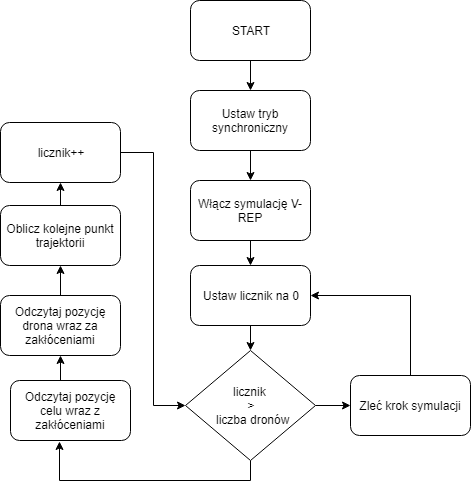
\includegraphics[scale=0.5]{uproszczony_digram_akcji.png}
\caption{Uproszczony diagram akcji.}

\end{figure}
Zadanie potymalizacji jest rozwiązywane przez funkcję fmincon(..).
\newpage
\section{Realizacja}
Docelowo został utworzony interfejs użytkownika(fig.4) umożliwiający zmianę parametrów symulacji m.in. maksymalne przyśpieszenie i prędkość ruchu dronów, odległość od celu zachowywaną przez drony po utworzeniu formacji oraz odległość pomiędzy sąsiednimi dronami a także wybór dostępnych formacji.

\begin{figure}[H]
\centering
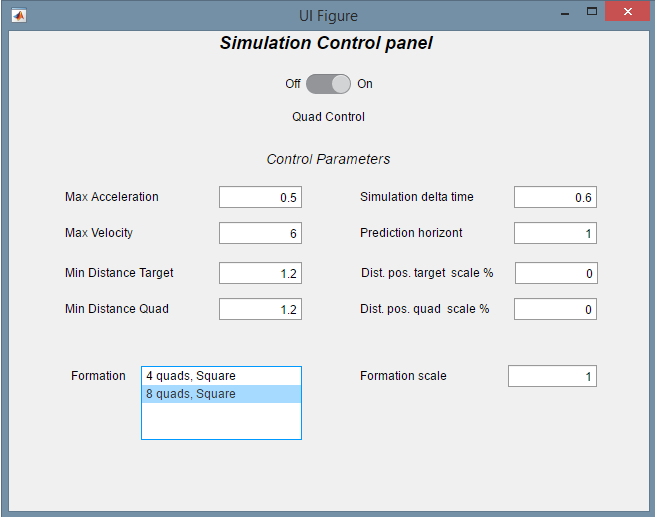
\includegraphics[scale=0.5]{interfejs.png}
\caption{Interfejs użytkownika.}
\end{figure}
Działanie zaimplementowanej optymalizacji dla czterech oraz ośmiu dronów, tworzących formację "kwadrat" nad celem, zostało przedstawione na poniższych rysunkach. Rysunki 5 i 7 przedstawiają początkowe położenie dronów oraz celu na planszy w programie V-rep. Natomiast Rysunki 6 i 8 przedstawiają utworzoną formacje nad przemieszczającym się człowiekiem.

\begin{figure}[H]
\centering
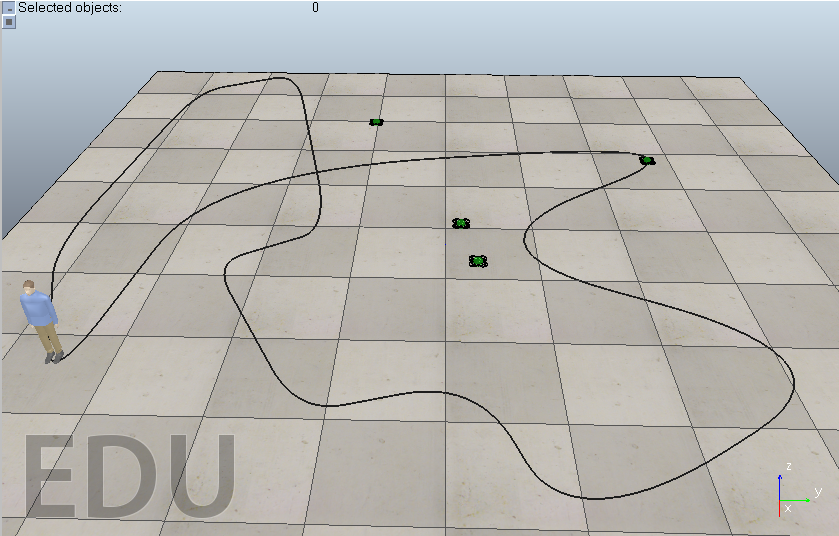
\includegraphics[scale=0.5]{sim_4_1.png}
\caption{Początkowe położenie dla symulacji czterech dronów.}
\end{figure}

\begin{figure}[H]
\centering
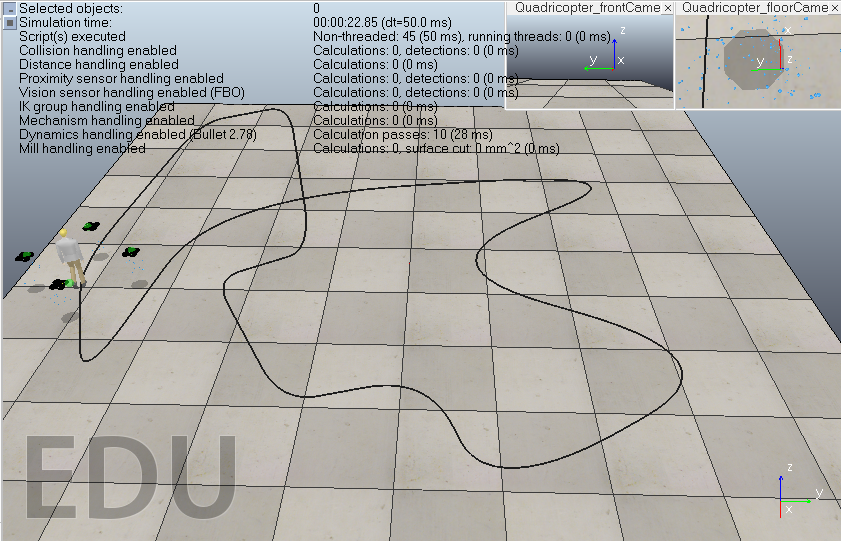
\includegraphics[scale=0.5]{sim_4_2.png}
\caption{Utworzona formacja dla czterech dronów.}
\end{figure}

\begin{figure}[H]
\centering
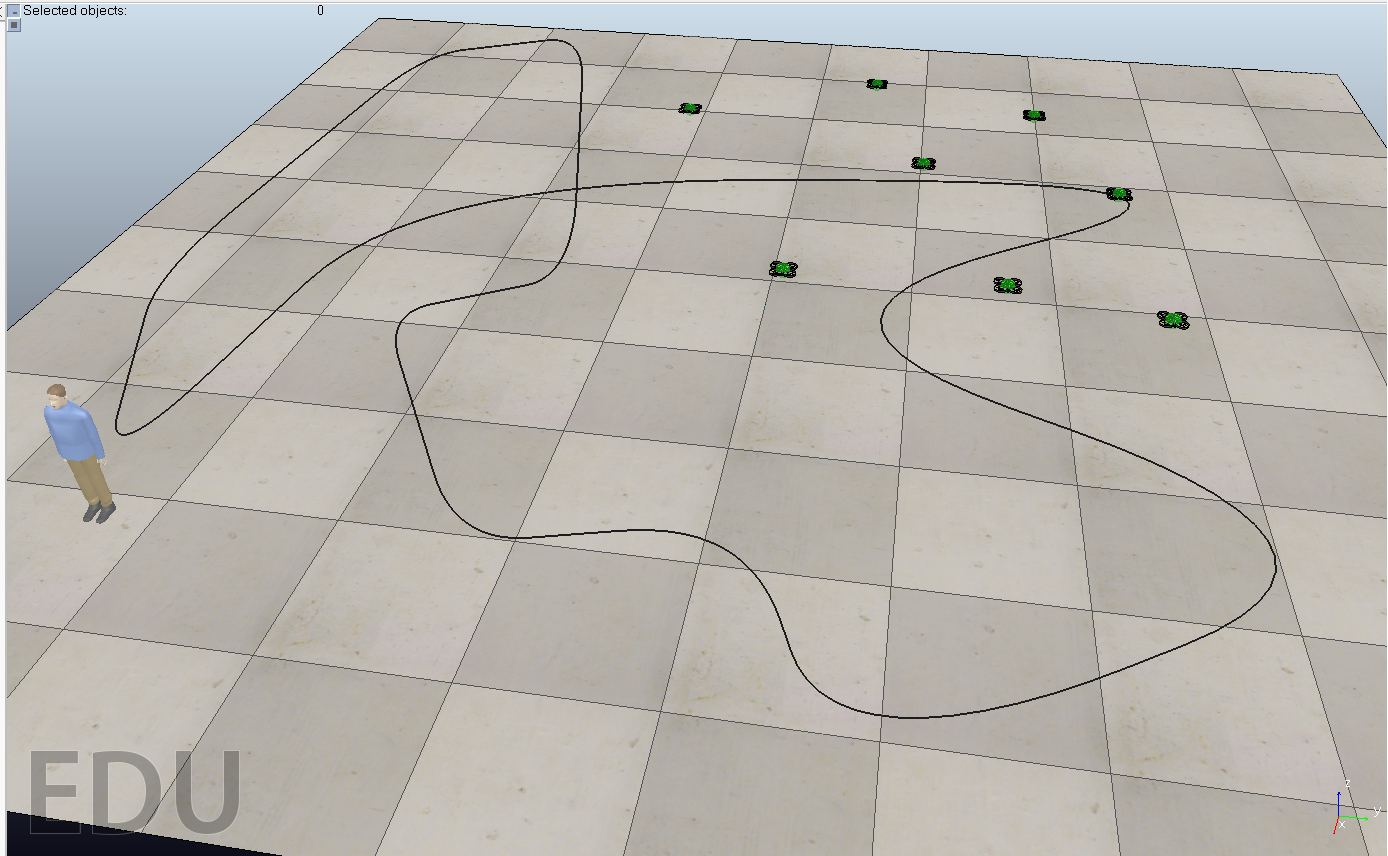
\includegraphics[scale=0.25]{sim_8_1.png}
\caption{Początkowe położenie dla symulacji ośmiu dronów.}
\end{figure}

\begin{figure}[H]
\centering
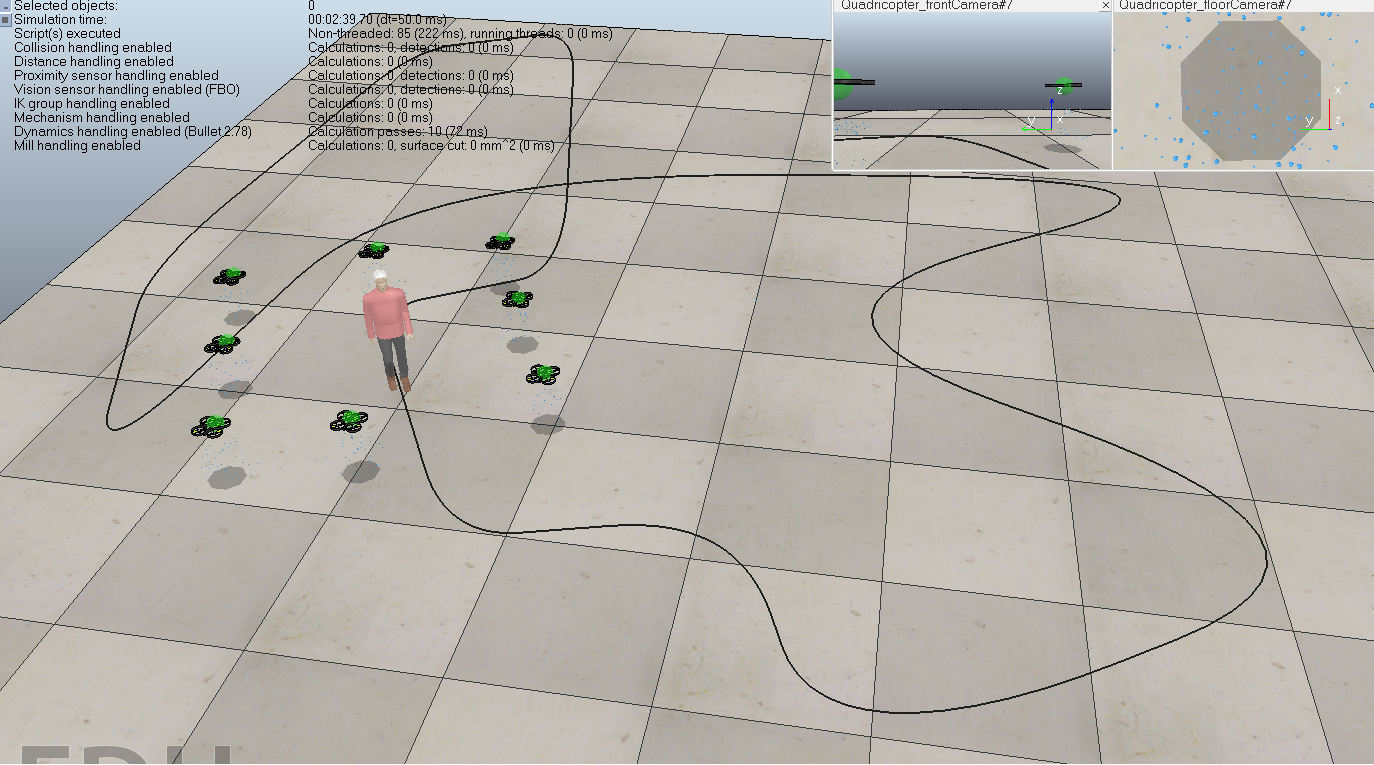
\includegraphics[scale=0.25]{sim_8_2.png}
\caption{Utworzona formacja dla ośmiu dronów.}
\end{figure}


\newpage
\section{Analiza rozwiązania}
W celu oceny poprawności oraz jakości zaimplementowanego zadania optymalizacji, wykreślono przebiegi w czasie, przedstawiające porównanie działania programu bez optymalizacji oraz po zastosowaniu optymalizacji. Pierwszy przebieg przedstawia sumaryczną drogę pokonaną przez każdego drona z pozycji początkowej do momentu utworzenia formacji nad celem. Można zauważyć, że po zastosowaniu optymalizacji znacznie skrócił się czas jaki jest potrzebny do utworzenia formacji z położenia początkowego. Drugą bardzo istotną korzyścią płynącą z zastosowania zadania optymalizacji, jest odległość przebyta przez drony. Po jej zastosowaniu dystans jaki jest potrzebny do utworzenia formacji nad celem zmalał o 30\%. 
\newline
Drugi przebieg przedstawia sumaryczne koszty energetyczne dla każdego statku, wykorzystywane  do utworzenia formacji z położenia początkowego. W tym przypadku również można zauważyć znaczną poprawę po zastosowaniu zadania optymalizacji. Koszty energetyczne są znacznie mniejsze, również zmalały o 30\% w stosunku do ruchu dronów bez zadania optymalizacji.   
\begin{figure}[H]
\centering
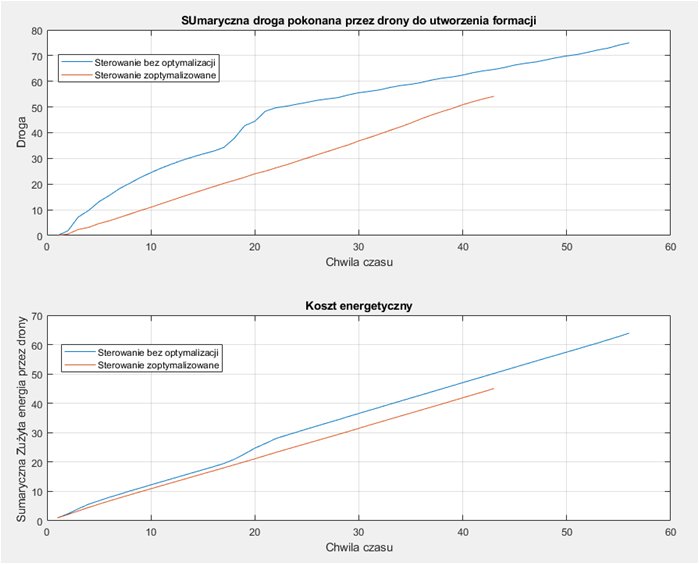
\includegraphics[scale=0.8]{porownanie.png}
\caption{Rezultaty przed i po zastosowaniu optymalizacji.}
\end{figure}


\newpage
\section{API}
Funkcja ConstraintFunction definiująca więzy narzucone na układ:
\newline
 $function [c,ceq]=ConstraintFunction(a,X,D_{min},d_{min},a_{0},v_{0},x_{0},t,V_{max},a_{max})$\newline
Parametry:
\begin{itemize}
\item $a$ -  minimalna odległość do sąsiada
\item $X$ - zmienna celu
\item $D_{min}$ -  minimalna odległość do celu
\item $d_{min}$ -  macierz minimalnych odległość od sąsiada
\item $a_{0}$ - początkowa odległość od sąsiada
\item $v_{0}$  - początkowa prędkość
\item $x_{0}$ - pozycja początkowa
\item $t$ - czas
\item $V_{max}$ - prędkość maksymalna
\item $a_{max}$ - największa, dopuszczalna odległość od sąsiada
\end{itemize}

Funkcja zwracająca pozycje celu.
\newline
$function Position = GetMainTrgtPos(VrepAPI, ClientID)$
\newline
Parametry:
\begin{itemize}
\item $VrepAPI$ - struktura zawierająca wszystkie funkcje dostępne w V-rep
\item $ClientID$ - identyfikator użytkownika
\end{itemize}

Funkcja zwracająca zakłóconą pozycje celu: 
\newline
$function [dpos, pos]=GetDisturbedMainTrgtPosition(VrepAPI, ClientID, scale)$
\newline
Parametry:
\begin{itemize}
\item $VrepAPI$ - struktura zawierająca wszystkie funkcje dostępne w V-rep
\item $ClientID$ - identyfikator użytkownika
\item $scale$ - współczynnik zakłócenia
\end{itemize}

Funkcja ustawiająca drony w pozycjach początkowych:
\newline
$function SetQuadTrgtPos(VrepAPI, ClientID, QuadNumber, Position)$
\newline
Parametry:
\begin{itemize}
\item $VrepAPI$ - struktura zawierająca wszystkie funkcje dostępne w V-rep
\item $ClientID$ -identyfikator użytkownika
\item $QuadNumber$ - numer drona dla którego aktualnie jest ustalana pozycja 
\item $Position$ - pozycja początkowa w układzie 2D
\end{itemize}
Funkcja zwracająca początkową pozycję dla każdego drona z zakłóceniem oraz bez zakłócenia:
\newline
$function [dpos, pos]=GetDisturbedQuadPosition(VrepAPI, ClientID, size, scale)$
\newline
Parametry:
\begin{itemize}
\item $VrepAPI$ - struktura zawierająca wszystkie funkcje dostępne w V-rep
\item $ClientID$ - identyfikator użytkownika
\item $size$ - liczba dronów 
\item $scale$ - współczynnik zakłócenia
\end{itemize}

Funkcja optymalizująca kolejne położenia dronów:
\newline
$function [a_x,a_y]=OptimizeNextMove(X,D,d,a_{0},v_{0},x_{0},t,D_{min},d_{min},V_{max},a_{max})$
\newline
Parametry:
\begin{itemize}
\item $X$ - zmienna celu
\item $D$ - odległość do celu
\item $d$ -  odległość od sąsiada
\item $a_{0}$ - początkowa odległość od sąsiada
\item $v_{0}$ - początkowa prędkość
\item $x_{0}$ - pozycja początkowa
\item $t$ -  czas
\item $D_{min}$ - minimalna odległość do celu
\item $d_{min}$ - minimalna odległość od sąsiada
\item $V_{max}$ - prędkość maksymalna
\item $a_{max}$ - największa, dopuszczalna odległość od sąsiada 
\end{itemize}

Funkcja zwracająca optymalną pozycje każdego z dronów oraz gradient sumaryczny zawierający gradient odległości od celu, gradient błędu utworzonej formacji oraz gradient prędkości poruszania się utworzonej formacji:
\newline 
$function [out,grad]=TargetFunction(a,X,D,d,v_{0},x_{0},t)$
\newline
Parametry:
\begin{itemize}
\item $a$ - minimalna odległość do sąsiada
\item $X$ - zmienna celu
\item $D$ - zadana odległość od celu 
\item $d$ - zadana macierz odległości do sąsiada
\item $v_{0}$ - początkowa prędkość
\item $x_{0}$ - pozycja początkowa
\item $t$ -  czas
\end{itemize}




\end{document}